\ifx\atempxetex\usewhat
\XeTeXinputencoding "utf-8"
\fi
\defaultfont

\chapter{内存管理}

对于一个进程来说,内存是最基本也是最重要的资源。这一章的内容是内存管理,包括:存储器分配(allocation),内存操控(manipulation)和最后的内存释放(release)。

动词“allocate”(获取内存的一般说法)有些误导人,因为它总是让人联想到分配一个稀缺的供不应求的资源。当然,每个用户都想拥有更多的内存。然而,在现代的操作系统中,问题的关键并不是是很多进程来共享很少的内存,而是如何适当的使用并跟踪使用情况。

在本章中,你将会学到在进程各个区段中分配内存的方法,以及各个方法的优缺点。我们也将会涉及一些设置和操作任意内存区域内容的方法,并了解如何把锁定内存,从而避免你的程序等待内核从交换区换页。 

\section{进程地址空间}

像所有的现代操作系统一样,Linux将它的物理内存虚拟化。进程并不能直接在物理内存上寻址,而是由Linux内核为每个进程维护一个特殊的虚拟地址空间(virtual address space)。这个地址空间是线性的,从0开始,到某个最大值。 

\subsection{页和页面调度}

虚拟空间由许多页组成。系统的体系结构以及机型决定了页的大小(页的大小是固定的),典型的页的大小包括4K(32位系统)和8K(64位系统)\footnote[1]{一些系统支持一系列的页面大小,由于这个原因,页面大小不是ABI(应用程序二进制接口)的一部分。应用程序必须在运行时获取页面大小,我们在第四章讨论过这个问题,本章我们将会加以回顾。}。每个页面都只有无效(invalid)和有效(valid)这两种状态,一个有效页面(valid page)和一个物理页或者一些二级存储介质相关联,例如一个交换分区或者一个在硬盘上的文件。一个无效页面(invalid page)没有关联,代表它没有被分配或使用。对无效页面的访问会引发一个段错误。地址空间不需要是连续的。虽然是线性编址,但实际上中间有很多未编址的小区域。

一个进程不能访问一个处在二级存储中的页,除非这个页和物理内存中的页相关联。如果一个进程尝试访问这样的页面,那么存储器管理单元(MMU)会产生一个页错误(page fault)。然后内核介会透明地从二级存储换入需要的页面。因为一般来说虚拟存储器总是要比物理内存大(在大多数系统上,在同一个虚拟地址空间中),所以内核也需要经常地把页面从物理内存换出(paging out)到二级存储,从而为将要换入的页面腾出空间。内核总是倾向于将未来最不可能使用的页换出,以此来优化性能。 

\subsubsection{共享和写时复制}

虚存中的多个页面,甚至是属于不同进程的虚拟地址空间,也有可能被映射到同一个物理页面。这样允许不同的虚拟地址空间共享(share)物理内存上的数据。共享的数据可能是只读的,或者是可读可写的。

当一个进程试图写某个共享的可写页时,可能发生以下两种情况之一。最简单的是内核允许这个操作,在这种情形下所有共享这个页的进程都将看到这次写操作的结果。通常,允许大量的进程对同一页面读写需要某种程度上的合作和同步机制。

而另一种情况是MMU会截取这次写操作并产生一个异常;作为回应,内核就会透明的创造一份这个页的拷贝以供该进程进行写操作。我们将这种方法称为写时拷贝(copy-on-write)(COW)\footnote[1]{回想第五章fork()就是使用了写时拷贝来使子进程共享父进程的地址空间。}。允许读取共享的数据可以有效的节省空间。当一个进程试图写一个共享页面时,可以立刻获得该页的一份拷贝,这使得内核工作起来就像每个进程都始终有它自己的私有拷贝。写时拷贝是以页为单位进行的,因此一个大文件可以有效的被众多进程共享。而每个进程只有在对共享页写时才能获得一份新的拷贝。 

\subsection{存储器区域}

内核将具有某些相同特征的页组织成块(blocks),例如读写权限。这些块叫做存储器区域(memory regions),段(segments),或者映射(mappings).下面是一些在每个进程都可以见到的存储器区域: 

\begin{itemize}
\item \begin{flushleft}文本段(text segment)包含着一个进程的代码,字符串,常量和一些只读的数据。在Linux中,文本段被标记为只读,并且直接从目标文件(可执行程序或是库文件)映射到内存中。\end{flushleft}
\item \begin{flushleft}堆栈段(stack)包括一个进程的执行栈,随着栈的深度动态的伸长或收缩。执行栈中包括了程序的局部变量(local variables)和函数的返回值。\end{flushleft}
\item \begin{flushleft}数据段(data segment),又叫堆(heap),包含着一个进程的动态存储空间。这个段是可写的, 而且它的大小是可以变化的。这部分空间往往是由malloc分配的(这将会在下一节讨论)。\end{flushleft}
\item \begin{flushleft}BSS段\footnote[1]{如此命名有一定的历史原因是从block started by symbol得到。}(bss segment)包含了没有被初始化的全局变量。这些变量根据不同的C标准都有特殊的值(通常来说,都是0)。

Linux从两个方面优化这些变量。首先,因为附加段是用来存放没有被初始化的数据的,所以链接器(ld)实际上并不会将特殊的值存储在对象文件中。这样可以减少二进制文件的大小。其次,当这个段被加载到内存时,内核只需简单的根据写时复制的原则将它们映射到一个全是0的页上,这样就十分有效的设置了这些变量的初始值。\end{flushleft}
\item \begin{flushleft}大多数地址空间含有很多映射文件,比如可执行文件自己,C或是其它的可链接库和数据文件。 可以看看/proc/self/maps,或者pmap程序的输出,我们能看到一个进程里面有很多的映像文件。\end{flushleft}
\end{itemize}

本章将介绍Linux提供的从如何获取内存到创建、销毁映射的各种接口。 

\section{动态内存分配}

内存同样可以通过自动变量和静态变量获得,但是所有内存管理系统的基础都是动态内存的分配,使用以及最终的返回。动态内存是在进程运行时才分配的,而不是在编译时就分配好了的,而分配的大小也只有在分配时才确定。作为一个程序员,当在程序运行前你不知道你需要多大的空间,或是你需要使用这块内存的时间不定,则需要使用动态内存。比如说,当你把一个文件或者用户从键盘的输入存到内存的时候。由于文件的大小以及用户输入内容的长度是不定的,因此缓冲区的大小是变化的,随着程序读到数据增多,应该它动态地增大内存。

C不提供支持动态内存的变量。例如,C不会提供在动态内存中获取结构体struct pirate\_ship的机制,而是提供了一种机制在动态内存中分配一个足够大空间来保存pirate\_ship。程序员通过一个指针来对这块内存进行操作,在这个例子中这个指针就是struct pirate\_ship*。

C中最经典的为获取动态内存的接口是malloc(): 

% \setmonofont{DejaVu Sans Mono}
\begin{lstlisting}
  #include <stdlib.h>
  void *malloc (size_t size);
\end{lstlisting}

成功调用malloc()时会得到一个size大小的内存区域,并返回一个指向这部分内存首地址的指针。这块内存区域的内容是未定义的,不要自认为全是0.失败时,malloc()返回NULL,并设置errno错误值为ENOMEM。

malloc()的使用简单明了,就像下面的例子。分配指定字节大小的内存: 

\begin{lstlisting}
  char *p;
  /* give me 2 KB! */
  p = malloc (2048);
  if (!p)
    perror ("malloc");
\end{lstlisting}

或者像这样,分配足够空间来存放一个结构体: 

\begin{lstlisting}
  struct treasure_map *map;
  /*
   * allocate enough memory to hold a treasure_map stucture
   * and point 'map' at it
   */
  map = malloc (sizeof (struct treasure_map));
  if (!map)
    perror ("malloc");
\end{lstlisting}

每次调用时,C都会自动地的把返回值由void指针转变为需要的类型。所以,这些例子在调用时并不需要将malloc()的返回值强转为一个左值类型。但是在C++并不提供这种自动的转换。因而,C++的使用者需要像下面一样对malloc()的返回值作强转: 

\begin{lstlisting}
  char *name;
  /* allocate 512 bytes */
  name = (char *) malloc (512);
  if (!name)
    perror ("malloc");
\end{lstlisting}

一些C的程序员喜欢将所有返回指针函数(包括malloc)的返回值强转为void。我非常反对这种行为,因为这之中隐含了一些问题。当函数的返回值变为其它不是void的指针时就会出错。更加严重的是,当一个函数不被正确声明的时候这样的强转会隐藏BUG\footnote[1]{没有声明的函数返回值默认是int类型的。Int到指针的强转并不是自动的,所以会产生警告。而强转会遮盖这个警告。}。如果说使用malloc时不会产生前一个问题,但后一个问题却很有可能发生。

因为malloc可以返回NULL,这对于那些习惯于检查错误的程序员来说是非常重要的。许多程序都定义和使用封装后的malloc(),当malloc()返回NULL时就打印错误和终止程序。根据约定,程序员们把这个封装叫作xmalloc():

\begin{lstlisting}
  /* like malloc(), but terminates on failure */
  void *xmalloc (size_t size)
  {
    void *p;
    p = malloc (size);
    if (!p) {
        perror ("xmalloc");
        exit (EXIT_FAILURE);
    }
    return p;
  }
\end{lstlisting}

\subsection{数组分配}

当所需分配的内存大小本身是可变的时,动态分配内存将更复杂。为数组分配动态内存是一个很好的例子。这时,数组元素的大小已经确定,但元素的个数却是变化的。为了便于处理这种情况,C 提供一个calloc()函数: 

% \setmonofont{DejaVu Sans Mono}
\begin{lstlisting}
  #include <stdlib.h>
  void *calloc (size_t nr, size_t size);
\end{lstlisting}

调用calloc()成功时会返回一个指针,指向一块可以存储下整个数组的内存(nr个元素,每个为size个字节)。所以,下面两种内存申请方式得到的内存大小是一样的(可能比请求的多,但不会少): 

\begin{lstlisting}
  int *x, *y;
  x = malloc (50 * sizeof (int));
  if (!x) {
          perror ("malloc");
          return -1;
  }
  y = calloc (50, sizeof (int));
  if (!y) {
          perror ("calloc");
          return -1;
  }
\end{lstlisting}

但两个函数的行为是有区别的。与malloc不同的是,calloc将分配的区域全部用0进行初始化。因此y中的50个元素都被赋值为0,但x数组里面的元素却是未定义的。如果程序不马上给这所有的50个元素赋值,程序员就应该使用calloc()来保证数组里面的元素不被莫名其妙的值填充。另外要注意的是二进制0和和浮点0是不一样的。

用户经常希望用0来初始化动态分配得到的内存,即使这内存不是用来存数组的。在这章的后面,我们会探讨memset函数,它提供了一个用指定的值填充指定内存块的接口。但是使用calloc会更快,因为内核可以提供本已清0的内存块。

当分配失败时,和malloc()一样,calloc()会返回NULL,并设置errno为ENOMEM。

我们不清楚为什么C标准不提供一个calloc以外的函数用来分配以及初始化。不过开发者可以很容易地定义他们自己的接口: 

\begin{lstlisting}
  /* works identically to malloc( ), but memory is zeroed */
  void *malloc0 (size_t size)
  {
    return calloc (1, size);
  }
\end{lstlisting}

另外我们可以非常方便的将malloc0和我们之前的xmalloc结合起来: 

\begin{lstlisting}
  /* like malloc( ), but zeros memory and terminates on failure */
  void *xmalloc0 (size_t size)
  {
    void *p;
    p = calloc (1, size);
    if (!p) {
            perror ("xmalloc0");
            exit (EXIT_FAILURE);
    }
    return p;
  }
\end{lstlisting}

\subsection{调整已分配内存大小}

C语言提供了一个接口来改变(变大或变小)已经得到的动态内存的大小:

% \setmonofont{DejaVu Sans Mono}
\begin{lstlisting}
  #include <stdlib.h>
  void *realloc (void *ptr, size_t size);
\end{lstlisting}

成功调用realloc()将ptr指向的内存区域的大小变为size字节。它返回一个指向新空间的指针,当试图扩大内存块的时候返回的指针可能不再是ptr。如果realloc不能在已有的空间上增加到size大小,那么就会另外申请一块size大小的空间,将原本的数据拷贝到新空间中,然后再将旧的空间释放。在任何情况,会根据新旧区域中的较小的一个来保留原来内存区域的内容。因为有潜在的拷贝操作,所以一个扩大原区域的realloc()操作可能是相当耗时的。

如果size是0,效果就会跟在ptr上调用free()相同。

如果ptr是NULL,结果就会跟malloc()一样。如果ptr是非NULL的,那么它必须是之前调用的malloc(), calloc(), 或realloc()之一的返回值。当失败的时候realloc()返回NULL并设置errno为ENOMEM。这时ptr指向的内存区域没有改变。

让我们探讨一下原存储区域收缩的情况。首先,我们会使用calloc()来申请足够的空间来存放一个由两个map结构组成的数组: struct map *p; 

\begin{lstlisting}
  /* allocate memory for two map structures */
  p = calloc (2, sizeof (struct map));
  if (!p) {
          perror ("calloc");
         return -1;
  }
  /* use p[0] and p[1]... */
\end{lstlisting}

现在我们已经达到目的了,所以我们决定修改内存块的大小,将一半的空间归还给系统(这可能不是一个非常有意义的操作,但当map结构非常大而我们剩下的那个map要保持很长时间时,这就变得有意义了):

\begin{lstlisting}
  /* we now need memory for only one map */
  r = realloc (p, sizeof (struct map));
  if (!r) {
          /* note that 'p' is still valid! */
          perror ("realloc");
          return -1;
  }
  /* use 'r'... */
  free (r);
\end{lstlisting}

在本例中,realloc()调用后,p[0]被保留了下来。所有的数据原封不动。如果realloc()失败了,由于p没有被改变,所以仍然是可用的。我们会继续使用它,直到最后释放这部分内存。另一方面,如果调用成功了,我们忽略p,并在这里使用r(看起来和p一样,只是指向的空间变小了)。当我们完成这一切的时候,要记得必须把r释放掉。 

\subsection{动态内存的释放}

自动内存分配,当栈不在使用,空间被自动释放。与之不同的是,动态内存将永久占有一个进程地址空间的一部分,直到它被显式地释放。因此,程序员们有责任将申请到的动态内存返回给系统。(当然,当整个进程都退出的时候,所有动态和静态的存储器都荡然无存了。)

当被malloc(), calloc(), 或者realloc()分配到的内存不再使用的时候必须通过free()归还给系统: 

% \setmonofont{DejaVu Sans Mono}
\begin{lstlisting}
  #include <stdlib.h>
  void free (void *ptr);
\end{lstlisting}

调用free()会释放ptr指向的内存。但ptr必须是之前调用malloc(), calloc(), 或者realloc()的返回值。也就是说,你不能用free()来释放申请到的部分内存,比如说用一个指针指向一块空间中间的位置。

ptr可能是NULL,这个时候free()什么都不做就返回了,因此调用free()时并不需要检查ptr是否为NULL。

让我们看看下面这个例子: 

\begin{lstlisting}
  void print_chars (int n, char c)
  {
    int i;
    for (i = 0; i < n; i++) {
        char *s;
        int j;
        /*
        * Allocate and zero an i+2 element array
        * of chars. Note that 'sizeof (char)'
        * is always 1.
        */
        s = calloc (i + 2, 1);
        if (!s) {
            perror ("calloc");
            break;
        }
        for (j = 0; j < i + 1; j++)
            s[j] = c;
        printf ("%s\n", s);
        /* Okay, all done. Hand back the memory. */
        free (s);
    }
  }
\end{lstlisting}

本例中,为n个字符数组分配了空间,n个数组的元素个数依次递增,从两个元素(2字节)一直到n+1个元素(n+1字节)。然后,循环将数组中的最后一个元素外的元素赋值为c(最后一个字节为0),之后将字符串打印,最后将s释放。 调用print\_chars(),让n等于5,c为X,我们可以得到如下图形: 

\begin{verbatim}
  X
  XX
  XXX
  XXXX
  XXXXX
\end{verbatim}

当然,还会有别的更有效率的方法来实现这个功能,但关键是,就算要分配的内存块的单元大小和个数要到运行时才确定,我们也可以动态的分配和释放内存。

\begin{wrapfigure}{l}{2.5cm}
  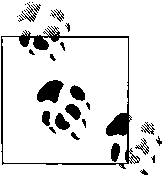
\includegraphics[width=2cm,clip]{paipai.png}
\end{wrapfigure}
\mbox{}\begin{flushleft}类似SunOS,SCO的Unix系统,提供一个free()的变种cfree(),它的行为跟具体的系统有关,有可能跟free()一 样,但也有可能接受三个参数,与calloc()相对.在Linux中,free()能处理我们现在涉及到的所有由动态存储机制分配到的内存。除非要考虑向下兼容的问题,不然我们不应该使用cfree()。所有Linux的版本中free()都是一样的。\end{flushleft}

要注意这个例子中如果不调用free()的结果。这个程序会永远也不将存储空间还给系统了,更为糟糕的是,唯一指向这块区域的指针s会消失,使得我们再也没有办法对这块内存进行操作。我们将这类编程错误叫做内存泄漏(memory leak)。内存泄漏以及其它一些动态内存产生的问题是很多程序中经常出现的,更不幸的是,这也是C语言编程中最可怕的小毛病。由于C语言将所有的内存管理交给程序员,所以程序员必须对于所有的内存分配格外注意。

另外一个最常见的错误是释放后再使用(use-after-free)。这个愚蠢的行为发生在一块内存被释放后,仍去访问它。一旦调用free()释放了某块内存,我们就再也不能对其进行操作了。程序员必须格外注意那些摇摆不定或指向不可使用内存块的指针。有两个常用的工具可以帮助你解决这些问题:Electric Fence和valgrind\footnote[1]{请见 http://perens.com/FreeSoftware/ElectricFence/ 以及 http://valgrind.org。}。

\subsection{对齐}

数据的对齐(alignment)是指数据地址和由硬件确定的内存块之间的关系。一个变量的地址是它大小的倍数时,就叫做自然对齐(naturally aligned)。例如,对于一个32bit长的变量,如果它的地址是4(字节)的倍数( 就是说,如果地址的低两位是0),那么这就是自然对齐了。所以,如果一个类型的大小是2n个字节,那么它的地址中,至少低n位是0。对齐的规则是根据硬件制定的。一些体系的计算机在数据对齐这方面有着很严格的要求。在有的系统中,载入一个没有对齐的数据将导致处理器的错误。在其它一些系统中,对不对齐的数据的访问是安全的,但却会引起性能的下降。在编写可移植的代码的时候,对齐的问题一定要注意,所有的类型都应该保持自然对齐。  

\subsubsection{预对齐内存的分配}

在大多数情况下,编译器和C库会自动处理对齐问题。POSIX规定通过malloc(),calloc()和realloc()返回的内存空间对于C中的标准类型都应该是对齐的。在Linux中,这些函数返回的地址在32位系统是以8字节为边界对齐,在64位系统是以16字节为边界对齐的。

有时候,对于更大的边界,例如页面,程序员需要动态的对齐。虽然动机是各不相同,但最基本的工作是将直接块I/O或是其它软硬件通信的缓冲区对齐。因此,POSIX 1003.1d提供一个叫做posix\_memalign()的函数: 

% \setmonofont{DejaVu Sans Mono}
\begin{lstlisting}
  /* one or the other -- either suffices */
  #define _XOPEN_SOURCE 600
  #define _GNU_SOURCE
  #include <stdlib.h>
  int posix_memalign (void **memptr,
                      size_t alignment,
                      size_t size);
\end{lstlisting}

调用posix\_memalign(),成功时会返回size字节的动态内存,并保证是按照alignment进行对齐的。参数alignment必须是2的幂,以及void指针大小的倍数。返回的内存块的地址保存在memptr里,函数返回0.

调用失败时,没有内存会被分配,memptr的值没有被定义,返回如下错误码之一: 

\begin{eqlist*}
\item[EINVAL] 参数不是2的幂,或者不是void指针的倍数。 
\item[ENOMEM] 没有足够的内存去满足函数的请求。 
\end{eqlist*}

要注意的是,对于这个函数,errno不会被设置,而是直接在返回值中给出。

由posix\_memalign()获得的内存通过free()释放。用法很简单: 

\begin{lstlisting}
  char *buf;
  int ret;
  /* allocate 1 KB along a 256-byte boundary */
  ret = posix_memalign (&buf, 256, 1024);
  if (ret) {
            fprintf(stderr, "posix_memalign: %s\n",
                     strerror (ret));
            return -1;
  }
  /* use 'buf'... */
  free (buf);
\end{lstlisting}

  更早的接口。在POSIX定义了posix\_memalign( )之前,BSD和SunOS分别提供了如下接口: 

% \setmonofont{DejaVu Sans Mono}
\begin{lstlisting}
  #include <malloc.h>
  void * valloc (size_t size);
  void * memalign (size_t boundary, size_t size);
\end{lstlisting}

函数valloc()的功能和malloc()一模一样,但返回的地址是页面对齐的。回顾一下第四章,页面的大小很容易通过getpagesize()得到。

相似地,函数memalign()是以boundary字节对齐的,而boundary必须是2的幂。在这个例子中,两个函数都返回一块足够大的内存去存放一个ship结构,并且地址都是在一个页面的边界上: 

\begin{lstlisting}
  struct ship *pirate, *hms;
  pirate = valloc (sizeof (struct ship));
  if (!pirate) {
               perror ("valloc");
               return -1;
  }
  hms = memalign (getpagesize ( ), sizeof (struct ship));
  if (!hms) {
            perror ("memalign");
            free (pirate);
            return -1;
  }
  /* use 'pirate' and 'hms'... */
  free (hms);
  free (pirate);
\end{lstlisting}

在Linux中,由这两个函数获得的内存都可以通过free()释放。但在别的Unix系统却未必是这样,一些系统并没有提供一个足够安全的机制来释放这些内存。出于移植性考虑,可能没有其他选择,但是注意不要使用free()去释放以上三个函数申请的内存。

只有为了移植到更老的系统上时,Linux的程序员才可以使用这两个函数。否则,应该优先选择posix\_memalign()。 这三个函数只有在malloc()的无法满足对齐需求时才使用。 

\subsubsection{其它对齐问题}

对齐问题不局限于标准类型与动态内存分配的自然对齐。比如说,复杂的数据类型的对齐问题将会比标准类型的更复杂。另外,在对不同类型的指针进行赋值以及强制类型转换的时候,对齐的问题也很重要。 

  非标准类型。非标准和复杂的数据类型的对齐比简单的自然对齐有着更多的要求。下面是四条有用的规则: 

\begin{itemize}
\item \begin{flushleft}一个结构的对齐要求和它的成员中最大的那个类型是一样的。例如,一个结构中最大的是以4字节对齐的32bit的整形,那么这个结构至少以4字节对齐。\end{flushleft}
\item \begin{flushleft}结构体也引入了对填充的需求,以此来保证每一个成员都符合各自的对齐要求。所以,如果一个char (可能以1字节对齐)后跟着一个int (可能以4字节对齐),编译器会自动地插入3个字节作为填充来保证int以4字节对齐。程序员们有时应该注意一下结构体中成员变量的顺序,来减少填充所导致的空间浪费。例如,可以将成员变量按照类型的大小进行排序。使用GCC编译时加入-Wpadded 选项可以帮助你应付这个问题。它会在填充时发出警告。\end{flushleft}
\item \begin{flushleft}一个联合的对齐和联合里最大的类型一致。 \end{flushleft}
\item \begin{flushleft}一个数组的对齐和数组里的元素类型一致。所以,除了对数组元素类型做对齐外,数组没有其他的对齐需求。这样可以使数组里面的所有成员都是自然对齐的。\end{flushleft}
\end{itemize}

  使用指针。因为编译器透明地处理了绝大多数的对齐问题,所以要找到潜在的错误的时候也比较困难。然而,这样的错误并不少见,特别是在处理指针和强转的时候。

假设一个指针从一个较少字节对齐的类型强转为一个较多字节对齐的类型,当通过这样的指针来访问时,会导致处理器不能对较多字节类型的数据正确对齐。例如,在如下的代码片段,c到badnews的强转使得程序将c当unsigned long来读: 

\begin{lstlisting}
  char greeting[] = "Ahoy Matey";
  char *c = greeting[1];
  unsigned long badnews = *(unsigned long *) c;
\end{lstlisting}

一个unsigned long 可能以4或8字节为边界对齐;而c当然只以1字节为边界对齐。因此当c被强转之后再进行读取将会导致对齐错误。这样的问题导致的后果,在不同的系统上各有不同,小者是性能损失,大者是整个程序崩溃。在可以发现而不能处理对齐错误的体系结构中,内核向出问题的进程发送SIGBUS信号来终止进程。我们会在第九章讨论信号。

像这样的例子在现实中出现的远远比你想的要多。当然现实中的例子肯定不会像这个一样明显,它们往往会更加隐蔽。 

\section{数据段的管理}

Unix系统在历史上提供过直接管理数据段的接口。然而,因为malloc()和其它的方法更强大也易于使用,大多数程序都不会直接地使用这些接口。我在这里说一下这些接口来满足一下大家的好奇心,同时也给那些想自己实现基于堆的动态分配机制的人一个参考: 

% \setmonofont{DejaVu Sans Mono}
\begin{lstlisting}
  #include <unistd.h>
  int brk (void *end);
  void * sbrk (intptr_t increment);
\end{lstlisting}

这些函数继承了一些老版本Unix系统中函数的名字,那时堆和栈还在同一个段中。堆中动态存储器的分配由数据段的底部向上生长;栈从数据段的顶部向着堆往下生长。堆和栈的分界线叫做中断(break)或中断点(break point)。在现代系统中,数据段存在于它自己的内存映射中,我们仍用中断点来标记映射的结束地址。

调用brk()会设置中断点(数据段的末端)的地址为end。在成功的时候,返回0。失败的时候,返回-1,并设置errno为ENOMEM。

调用sbrk()将数据段末端增加increment字节,increment可正可负。sbrk()返回修改后的断点。所以,increment为0时得到的是现在断点的地址: 

\begin{lstlisting}
  printf("The current break point is %p\n",sbrk(0));
\end{lstlisting}

尽管POSIX和C都没有定义这些函数。但几乎所有的Unix系统都至少支持其中之一。可移植的程序应该坚持使用基于标准的接口。 

\section{匿名存储器映射}

glibc的内存分配使用了数据段和内存映射。实现malloc( )最经典方法就是将数据段分为一系列的大小为2的幂的块,返回最小的符合要求的那个块来满足请求。释放则只是简单的将这块区域标记为未使用。如果相邻的分区都是空闲的,他们会被合成一个更大的分区。如果堆的最顶端是空的,系统可以用brk( )来降低断点,使堆收缩,将内存返回给系统。

这个算法叫做伙伴内存分配算法(buddy memory allocation scheme)。它的优点是高速和简单,缺点则是会产生两种类型的碎片。当使用的内存块大于请求的大小时则产生内部碎片(Internal fragmentation)。这导致了内存的低使用率。外部碎片是在空闲存储器合计起来足够满足一个请求,但是没有一个单独的空间块可以来处理这个请求时发生的。这同样会导致内存利用不足(因为可能会分配一个更大的块)或是分配的失败(如果已经没有可选的块存在了)。

另外,这个算法会使一个内存的分配“栓”住另外一个,导致glibc不能将释放的内存返回给系统。想象内存中已被分配的两个块,块A和块B。块A正好处在中断点的位置,块B刚好在A的下面,就算释放了B,在A被释放前,glibc也不能相应的调整中断点。在这种情况下,一个长期存在的内存分配就把另外的空闲空间“栓”住了。

不过不必为此担忧,因为glibc并不是一直在试图将空间返回给系统\footnote[1]{glibc也使用比这伙伴系统更加先进的存储分配算法,叫做arena 算法。}。通常来说,在每次释放后堆并不收缩。glibc会维护释放的内存以供之后的分配使用。只有当堆明显的大于已分配的内存时,glibc才会减小数据段的大小。从另一方面看,一个较大的分配会阻止这种收缩。 

因此,对于较大的分配,glibc并不使用堆而是创建一个匿名内存映射(anonymous memory mapping)来满足要求。匿名存储器映射和在第四章讨论的基于文件的映射很相似,只是它并不基于文件-所以称之为“匿名”。实际上,一个匿名内存映射只是一块已经用0初始化的大的内存块,以供用户使用。可以把它想成为单独为某次分配而使用的堆。因为这种映射的存储不是基于堆的,所以并不会在数据段内产生碎片。

使用匿名映射来分配内存有下列好处: 

\begin{itemize}
\item \begin{flushleft}无需关心碎片。当程序不再需要这块内存的时候,只要撤销映射,这块内存就直接归还给系统了。\end{flushleft}
\item \begin{flushleft}匿名存储映射的大小的是可调整的,可以设置权限,还能像普通的映射一样接受建议(看第四章)。\end{flushleft}
\item \begin{flushleft}每个分配存在于独立的内存映射。没有必要再去管理一个全局的堆了。\end{flushleft}
\end{itemize}

使用匿名映射与堆比起来也有两个缺点: 

\begin{itemize}
\item \begin{flushleft}每个存储器映射都是页面大小的整数倍。所以,如果大小不是页面整数倍的分配会浪费大量的空间。对于较小的分配来说,空间的浪费更加显著,因为相对于使用的空间,浪费的空间将更大。\end{flushleft}
\item \begin{flushleft}创建一个新的内存映射比从堆中返回内存的负载要大,因为使用堆几乎不涉及任何内核操作。越小的分配,这样的问题也越明显。\end{flushleft}
\end{itemize}

根据各自的优缺点来判断,glibc的malloc() 使用数据段来满足小的分配,而匿名内存映射则用来满足大的分配。两者的临界点是可调的(请参阅本章稍后的高级内存分配部分),并会随着glibc版本的不同而有所变化。目前,临界点一般是128KB:比128KB小的分配由堆实现,相应地,较大的由匿名存储器映射来实现。 

\subsection{创建匿名存储器映射}

或许你在某次分配想要使用一个内存映射而不是堆,又或者你正在写自己的内存分配系统,想要手工创建自己的匿名内存映射,不管怎么样,Linux都将让它变得非常简单。回忆一下第四章,用mmap()函数来创建内存映射,而用munmap()来销毁: 

% \setmonofont{DejaVu Sans Mono}
\begin{lstlisting}
  #include <sys/mman.h>
  void * mmap (void *start,
               size_t length,
               int prot,
               int flags,
               int fd,
               off_t offset);
  int munmap (void *start, size_t length);
\end{lstlisting}

因为不需要打开和管理文件,创建匿名存储器映射要比创建基于文件的存储器映射更简单。两者最关键的差别在于是否有匿名标记。让我们来看看这个例子: 

\begin{lstlisting}
  void *p;
  p = mmap (NULL, /* do not care where */
            512 * 1024, /* 512 KB */
            PROT_READ | PROT_WRITE, /* read/write */
            MAP_ANONYMOUS | MAP_PRIVATE, /* anonymous, private */
            -1, /* fd (ignored) */
            0); /* offset (ignored) */
  if (p == MAP_FAILED)
        perror ("mmap");
  else
        /* 'p' points at 512 KB of anonymous memory... */
\end{lstlisting}

对于大多数的匿名映射来说,mmap()的参数都跟这个例子一样。当然了,需要程序员确定映射大小的参数。其他参数大致如下: 

\begin{itemize}
\item \begin{flushleft}第一个参数是start,被设为NULL,意味着匿名映射可以让内核安排的在任意地址上。当然给定一个non-NULL值也是可以的,只要它是页对齐的,但这样会限制了可移植性。实际上很少有程序真正在意映射到哪个地址上去!\end{flushleft}
\item \begin{flushleft}prot参数经常都同时设置了PROT\_READ和PROT\_WRITE位,使得映射是可读可写的。一块不能读写的空存储器映射是没有用的。另外一方面,很少将可执行代码映射到匿名映射,因为那样做能产生潜在的安全漏洞。 \end{flushleft}
\item \begin{flushleft}flags参数设置MAP\_ANONYMOUS位,来使得映射是匿名的,设置MAP\_PRIVATE位,使得映射是私有的。 \end{flushleft}
\item \begin{flushleft}假如MAP\_ANONYMOUS被设置了,fd和offset参数将被忽略的。然而,在一些更早的系统里,需要让fd为-1,因此如果要考虑到程序的可移植性,那么这是一个好主意。 \end{flushleft}
\end{itemize}

匿名映射获得的内存块,看上去和由堆获得的一样。通过匿名映射进行分配的一个好处是所有的页都已经用0进行了初始化。由于内核使用写时复制(copy-on-write)将内存块映射到了一个全0的页面上,因而避免了额外的开销。同时也就没有必要对返回的内存块使用memset()。事实上这就是使用calloc()比先使用malloc()再使用memset()效果要好的原因之一:glibc知道匿名映射是本来就全0的了,使用该映射的calloc()则不需要再显式的置零了。系统调用munmap()释放一个匿名映射,归还已分配的内存给内核。 

\begin{lstlisting}
  int ret;
  /* all done with 'p', so give back the 512 KB mapping */
  ret = munmap (p, 512 * 1024);
  if (ret)
  perror ("munmap");
\end{lstlisting}

\begin{wrapfigure}{l}{2cm}
  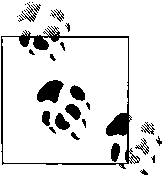
\includegraphics[width=1.5cm,clip]{paipai.png}
\end{wrapfigure}
\mbox{}\begin{flushleft}想复习一下mmap(),munmap(),和一般的映射,请参阅第四章。\end{flushleft}


\subsection{映射到/dev/zero}

其它Unix系统(例如BSD),并没有MAP\_ANONYMOUS标记。相反,它们使用特殊的设备文件/dev/zero实现了一个类似的解决方案。这个设备文件提供了和匿名内存相同的语义。一个包含全0的写时复制页面的映射;因此其行为和匿名存储器一致。 Linux一直支持/dev/zero设备,可以通过映射这个文件来获得全0的内存块。实际上,在引入MAP\_ANONYMOUS之前,Linux的程序员就使用该方法。为了对早期的Linux版本提供向下兼容或是为了移植到其它Unix系统上,程序员仍然可以将/dev/zero作为匿名映射替代方案。这与其他文件的映射没什么区别: 

\begin{lstlisting}
  void *p;
  int fd;
  /* open /dev/zero for reading and writing */
  fd = open ("/dev/zero", O_RDWR);
  if (fd < 0) {
              perror ("open");
              return -1;
  }
  /* map [0,page size) of /dev/zero */
  p = mmap (NULL, /* do not care where */
            getpagesize ( ), /* map one page */
            PROT_READ | PROT_WRITE, /* map read/write */
            MAP_PRIVATE, /* private mapping */
            fd, /* map /dev/zero */
            0); /* no offset */
  if (p == MAP_FAILED) {
                       perror ("mmap");
                       if (close (fd))
                       perror ("close");
                       return -1;
  }
  /* close /dev/zero, no longer needed */
  if (close (fd))
      perror ("close");
  /* 'p' points at one page of memory, use it... */ 
\end{lstlisting}

采用这种映射方式的存储器当然也是用munmap()来取消映射的。

然而这种方法因为要打开和关闭设备文件,所以会有额外的调用开销。因此匿名内存映射是一种较快的方法。 

\section{高级存储器分配}

本章所涉及的许多存储分配操作都是为内核的参数所控制和限制的,但程序员可以修改这些参数。为此,可以使用mallopt()函数: 

% \setmonofont{DejaVu Sans Mono}
\begin{lstlisting}
#include <malloc.h>
int mallopt (int param, int value);
\end{lstlisting}

调用mallopt()会将由param确定的存储管理相关的参数设为value。成功时,调用返回一个非0值;失败时,返回0。一般来说它都会正常返回,所以不要对能从返回值中获得什么抱太大的希望。

Linux目前支持六种param值,均被定义在了<malloc.h>中: 


\begin{eqlist*}
\item[M\_CHECK\_ACTION]环境变量MALLOC\_CHECK\_的值(将在下一节讨论)。 
\item[M\_MMAP\_MAX]系统用来满足动态存储器请求的最大存储器映射数。当达到这个限制时,分配就只能在数据段中进行,直到其中一个映射被释放。当该值为0时将禁止匿名映射用于动态存储的分配。 
\item[M\_MMAP\_THRESHOLD]决定该用匿名映射还是用数据段来满足存储器分配请求的阈值(以字节为单位)。要注意的是,有时候系统为了慎重起见,就算是比临界值小,也有可能用匿名映射来满足动态存储器的分配。值为0时会启用匿名映射来满足所有的分配,而不再使用数据段来满足请求。 
\item[M\_MXFAST]Fast bin的最大大小(以字节为单位)。Fast bins是堆中特殊的内存块,永远不和临近的内存块合并,也永远不归还给系统,以增加碎片为代价来满足高速的内存分配。值为0时,fasy bin将不被启用。 
\item[M\_TOP\_PAD]调整数据段的长度而使用的填充(padding)字节数。当glibc通过brk()来增加数据段的大小时,它可能申请更多的内存,希望减少很快再次调用brk()的可能性。相似地,但glibc收缩数据段的时候,它会保持一些多余的内存,而不是将所有的归还给系统。这多余的部分就称为填充。值为0时会取消使用填充。 
\end{eqlist*}

XPG中定义了mallopt(),并指定了另外三个参数:M\_GRAIN, M\_KEEP, 和M\_NLBLKS。Linux中定义了这些参数,但是实际上不起任何作用。表8-1定义了所有合法参数,他们的缺省值以及可接受的范围。 

\begin{center}
\begin{tabular}{ccccc}
  \toprule [1pt]
  \rowcolor[gray]{.9}
    参数 & 来源 & 缺省值 & 有效范围 & 特殊值来源 \\
  \midrule
    M\_CHECK\_ACTION & Linux特有 & 0 & 0-2 & 无 \\
	M\_GRAIN & XPG标准 & Linux不支持 & >=0 & 无 \\
	M\_KEEP & XPG标准 & Linux不支持 & >=0 & 无 \\
	M\_MMAP\_MAX & Linux特有 & 64*1024 & >=0 & 0禁用mmap() \\
	M\_MMAP\_THRESHOLD & Linux特有 & 128*1024 & >=0 & 0禁用堆 \\
	M\_MXFAST & XPG标准 & 64 & 0-80 & 0禁用fast bin \\
	M\_NLBLK & XPG标准 & Linux不支持 & >=0 & 无 \\
	M\_TOP\_PAD & Linux特有 & 0 & >=0 & 0禁用填充 \\
  \bottomrule[1pt]
\end{tabular}
\end{center}

程序必须要在调用malloc()或是其它内存分配函数前使用mallopt(),使用方法也非常简单: 

\begin{lstlisting}
  /* use mmap( ) for all allocations over 64 KB */
  ret = mallopt (M_MMAP_THRESHOLD, 64 * 1024);
  if (!ret)
      fprintf (stderr, "mallopt failed!\n");
\end{lstlisting}

\subsection{使用malloc\_usable\_size()和malloc\_trim()进行调优}

Linux提供了两个用来控制glibc内存分配系统的底层函数。第一个此类函数允许程序查询一块已分配内存中有多少可用字节: 

% \setmonofont{DejaVu Sans Mono}
\begin{lstlisting}
  #include <malloc.h>
  size_t malloc_usable_size (void *ptr);
\end{lstlisting}

调用malloc\_usable\_size()成功时,返回ptr指向的动态内存块的实际大小。因为glibc可能扩大动态内存来适应一个已存在的块或匿名映射,动态存储器分配中的可使用空间可能会比请求的大。当然,永远不可能比请求的小。下面是一个使用这个函数的例子: 

\begin{lstlisting}
  size_t len = 21;
  size_t size;
  char *buf;
  buf = malloc (len);
  if (!buf) {
            perror ("malloc");
            return -1;
  }
  size = malloc_usable_size (buf);
  /* we can actually use 'size' bytes of 'buf'... */
\end{lstlisting}

第二个函数允许程序强制glibc归还所有的可释放的动态内存给内核: 

 % \setmonofont{DejaVu Sans Mono}
\begin{lstlisting}
  #include <malloc.h>
  int malloc_trim (size_t padding);
\end{lstlisting}

调用malloc\_trim()成功时,数据段会尽可能地收缩,但是填充字节被保留下来。然后返回1。失败时,返回0。一般来说,每当空闲的内存到达M\_TRIM\_THRESHOLD 字节时,glibc会自动做这种收缩。使用M\_TOP\_PAD来用作填充。你不应该将这两个函数用于调试和教学以外的其它地方。它们是不可移植的,而且会将glibc内存分配系统的一些底层细节暴露给你的程序。 

\section{调试内存分配}

程序可以设置MALLOC\_CHECK\_环境变量来开启存储系统额外的调试功能。这个额外的调试检查是以降低内存分配的效率为代价的,然而这个开销在开发应用的调试阶段却是非常值得的。

因为仅仅一个环境变量就能控制调试,你不必重新编译你的程序。例如,你可以简单的执行如下指令: 

\begin{lstlisting}
$ MALLOC_CHECK_=1 ./rudder
\end{lstlisting}

如果设置为0,存储系统会忽略所有错误。如果它被设为1了,信息会被输出到标准错误输出stderr。如果设置为2,进程会立即通过abort( )终止。因为 MALLOC\_CHECK\_ 会改变正在运行的程序的行为,所以setuid程序忽略这个变量。 

\subsection{获得统计数据}

Linux提供了mallinfo()函数来获得关于动态存储分配系统的统计数据: 

% \setmonofont{DejaVu Sans Mono}
\begin{lstlisting}
  #include <malloc.h>
  struct mallinfo mallinfo (void);
\end{lstlisting}

mallinfo()的调用将统计数据保存到mallinfo结构中。这个结构是通过值而不是指针返回的。它的字段结构也在<malloc.h>定义了。

\begin{lstlisting}
  /* all sizes in bytes */
  struct mallinfo {
     int arena; /* malloc使用的数据段的大小 */
     int ordblks; /* 空闲块的个数 */
     int smblks; /* fast bin 的个数 */
     int hblks; /* 匿名映射的个数 */
     int hblkhd; /* 匿名映射的大小 */
     int usmblks; /* 最大已分配值 */
     int fsmblks; /* 可用的fast bin的大小 */
     int uordblks; /* 所有的被分配的空间 */
     int fordblks; /* 可用的块大小 */
     int keepcost; /* 可消去的多余空间的大小 */};
\end{lstlisting}


用法很简单: 

\begin{lstlisting}
  struct mallinfo m;
  m = mallinfo();
  printf ("free chunks: %d\n", m.ordblks);
\end{lstlisting}

Linux 也提供了malloc\_stats()函数,将跟内存相关的统计数据打印到标准错误输出(stderr): 

% \setmonofont{DejaVu Sans Mono}
\begin{lstlisting}
  #include <malloc.h>
  void malloc_stats (void);
\end{lstlisting}

在内存操作频繁的程序中调用往往会产生一些较大的数字: 

\begin{verbatim}
  Arena 0:
  system bytes = 865939456
  in use bytes = 851988200
  Total (incl. mmap):
  system bytes = 3216519168
  in use bytes = 3202567912
  max mmap regions = 65536
  max mmap bytes = 2350579712
\end{verbatim}

\section{基于栈的分配}

到目前为止,我们学过的所有的动态内存分配机制都是使用堆和存储器映射来实现的。我们很自然的想到使用它们因为堆和匿名映射本身就是动态的。另外一个在程序地址空间中常用的结构,栈,是用来存放程序的自动变量(automatic variables)的。

然而,认为程序员不能使用栈来进行动态内存分配是毫无理由的。只要一个分配不使栈溢出,这样的做法是简单而完美的。如果要在一个栈中实现动态内存分配,使用系统调用alloca():

% \setmonofont{DejaVu Sans Mono}
\begin{lstlisting}
  #include <alloca.h>
  void * alloca (size_t size);
\end{lstlisting}

调用alloca(),成功时会返回一个指向size字节大小的内存指针。这块内存是在栈中的,当调用它的函数(例如main函数)返回时,这块内存将被自动释放。某些该函数的实现会在失败时返回NULL,但是大部分时候alloca()都不可能失败,或是不可能报告失败。失败就表明出现的栈溢出。

用法与malloc()一样,但你不必(实际上,是不能)释放分配到的内存。以下示例函数,在系统配置目录(可能是/etc) 里面打开一个给定的文件,目录在编译时就被确定了。这个函数必须申请一个新的缓冲区,复制系统配置路径到这个缓冲区里面,然后将提供的文件名拼接到缓冲区的后面: 

\begin{lstlisting}
  int open_sysconf (const char *file, int flags, int mode)
  {
    const char *etc = SYSCONF_DIR; /* "/etc/" */
    char *name;
    name = alloca (strlen (etc) + strlen (file) + 1);
    strcpy (name, etc);
    strcat (name, file);
    return open (name, flags, mode);
  }
\end{lstlisting}

在open\_sysconf函数返回时,从alloca()分配到的内存随着栈的收缩而被自动释放。这意味着当调用alloca()的函数返回后,你不能再使用由alloca()得到的那块内存!然而,你并不需要做任何释放工作,所以最终代码会简洁一些。下面是一个通过malloc()实现的相同的函数: 

\begin{lstlisting}
  int open_sysconf (const char *file, int flags, int mode)
  {
      const char *etc = SYSCONF_DIR; /* "/etc/" */
      char *name;
      int fd;
      name = malloc (strlen (etc) + strlen (file) + 1);
      if (!name) {
                 perror ("malloc");
                 return -1;
      }
      strcpy (name, etc);
      strcat (name, file);
      fd = open (name, flags, mode);
      free (name);
      return fd;
  }
\end{lstlisting}

要注意的是你不能使用由alloca()得到的内存来作为一个函数调用的参数,因为分配到的内存块会被当做参数保存在函数的栈中。例如,下面这样做是不行的: 

\begin{lstlisting}
  /* DO NOT DO THIS! */
  ret = foo (x, alloca (10));
\end{lstlisting}

alloca() 接口有着曲折的历史。在许多系统,它表现得非常差,或者出现没被定义的行为。在栈大小较小而且是确定的系统中,使用alloca()很容易出现栈溢出,导致程序崩溃。在另外一些系统中,alloca()甚至就不存在。由于经常出错和不稳定,人们对alloca()总是没有一个好的印象。

所以,如果要让代码具有可移植性,你要避免使用alloca()。然而在Linux系统上,alloca()却是一个非常好用但没有被人们认识到的工具。它表现的异常出色(在各种架构下,通过alloca()进行内存分配就和增加栈指针一样简单),比malloc()的性能要好很多。对于Linux下较小的内存分配,alloca()能收获让人激动的性能。 

\subsection{栈中的复制串}

alloca()常见的用法是用来临时复制一个字符串。例如: 

\begin{lstlisting}
  /* we want to duplicate 'song' */
  char *dup;
  dup = alloca (strlen (song) + 1);
  strcpy (dup, song);
  /* manipulate 'dup'... */
  return; /* 'dup' is automatically freed */
\end{lstlisting}

因为这种需求非常多以及alloca()实现的高效,Linux系统专门提供了strdup()来将一个给定的字符串复制到栈中: 

% \setmonofont{DejaVu Sans Mono}
\begin{lstlisting}
  #define _GNU_SOURCE
  #include <string.h>
  char * strdupa (const char *s);
  char * strndupa (const char *s, size_t n);
\end{lstlisting}

调用strdupa( )会返回一个s的拷贝。strndupa()将拷贝s中的n个字符。如果s长度大于n,就复制s前n个字节,然后后面自动加上一个空字节。这些函数具有alloca()的优点。当调用函数返回时,复制的串会自动释放。 POSIX并没有定义alloca( ), strdupa( ),或者strndupa( )函数,它们在别的操作系统的表现也差强人意。如果考虑到可移植性,不鼓励使用这些函数。然而在Linux上,alloca()以及由它衍生的一些函数却表现的非常好,可以通过简单的移动栈指针来代替其它一些复杂动态分配内存方法,从而带来性能上的提升。

\subsection{变长数组}

C99 引进了变长数组(VLAs),变长数组的长度是在运行时决定的,而不是在编译的时候。。在这之前,GNUC已经支持变长数组了,但是现在C99将其标准化,因此对于变长数组的使用得到了很大的鼓励。VLAs用与alloca()相似的方法避免了动态存储分配所产生的负载。它的使用方法就跟你想象的一样: 

\begin{lstlisting}
  for (i = 0; i < n; ++i) {
      char foo[i + 1];
      /* use 'foo'... */
  }
\end{lstlisting}

在这个代码片段中,foo是一个有i+1个char的数组。在每次循中,foo都被动态的创建,并在这轮循环结束时自动释放。如果我们使用alloca()来代替VLA,那么内存空间将直到函数返回时才会被释放。使用一个VLA确保了内存每次循环都被释放。所以,使用VLA最多使用n个字节,而alloca()会使用掉n*(n+1)/2个字节。使用一个变长数组,我们能够像这样重写我们的open\_sysconf()函数: 

\begin{lstlisting}
  int open_sysconf (const char *file, int flags, int mode)
  {
      const char *etc; = SYSCONF_DIR; /* "/etc/" */
      char name[strlen (etc) + strlen (file) + 1];
      strcpy (name, etc);
      strcat (name, file);
      return open (name, flags, mode);
  }
\end{lstlisting}

alloca()和变长数组的主要区别在于通过前者获得的内存在函数执行过程中始终存在,而通过后者获得的内存在出了作用域后便释放了。这样的方式有好有坏。在for循环中,我们希望每次循环都能释放空间以在没有任何副作用的情况下减小内存的开销(我们不会希望有多余的内存始终被占用着)。然而,如果出于某种原因我们希望这块空间能保留到下一轮的循环中,那么使用alloca()显然是更加合理的。

\begin{wrapfigure}{l}{2.5cm}
  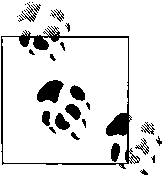
\includegraphics[width=2cm,clip]{paipai.png}
\end{wrapfigure}
\mbox{}\begin{flushleft}在单个函数中混淆了alloca()和变长数组会给程序引入怪异的行为。因此为了安全起见在一个固定的函数中只应使用其中之一。 \end{flushleft}

\section{选择一个合适的内存分配机制}

本章中讨论了很多种内存分配的方式,这可能使得程序员们不清楚在一个具体的问题中到底该使用哪一种。在大部分的情况下malloc()总是最好的选择。然而在某些情况下,采用其它方法会更好一些。表8-2总结了一些选择内存分配机理的原则: 

\begin{center}
\begin{tabular}{p{3cm}p{5cm}p{5cm}}
  \toprule [1pt]
  \rowcolor[gray]{.9}
    分配方式 & 优点 & 缺点 \\
  \midrule
    malloc() & 简单,方便,最常用 & 返回的内存为用零初始化   \\
    calloc() & 使数组分配变得容易,
	
	用0初始化了内存 & 在分配非数组空间时显得较复杂   \\
    realloc() & 调整已分配的空间大小 & 只能用来调整已分配空间的大小  \\
    brk()和sbrk() & 允许对堆进行深入控制 & 对大多数使用者来说过于底层  \\
    匿名内存映射 & 使用简单,可共享,允许开发者调整保护等级并提供建议,适合大空间的分配 & 不适合小分配。最优时malloc()会自动使用匿名内存映射 \\
    posix\_memalign() & 分配的内存按照任何合理的大小进行对齐 & 相对较新,因此可移植性是一个问题;对于对齐的要求不是很迫切的时候,则没有必要使用\\
    memalign()和valloc() & 相比posix\_memalign()在其它的Unix系统上更常见 & 不是POSIX标准,对对齐的控制能力不如posix\_memalign() \\
    alloca() & 最快的分配方式,不需要知道确切的大小,对于小的分配非常适合 & 不能返回错误信息,不适合大分配,在一些Unix系统上表现不好 \\
    变长数组 & 与alloca()类似,但在退出此层循环是释放空间,而不是函数返回时 & 只能用来分配数组,在一些情况下alloca()的释放方式更加适用,在其它Unix系统中没有alloca()常见 \\
  \bottomrule[1pt]
\end{tabular}
\end{center}

最后我们不能忘记以上方式之外的两个选择: 静态分配和自动分配。在栈中分配临时变量以及在堆中分配全局变量总是最简单的,而且不需要程序员们控制指针以及释放内存。 

\section{存储器操作}

C语言提供了很多函数进行内存操作。这些函数的功能和字符串操作函数(如strcmp()以及strcpy())类似,但是他们处理的对象是用户提供的内存区域而不是以NULL结尾的字符串。要注意这些函数都不会返回错误信息。因此防范错误是程序员的责任,如果传递错误的内存区域作参数的话,你将毫无疑问的得到段错误。 

\subsection{字节设置}

在一系列的内存操作函数当中,最常用的是memset(): 

% \setmonofont{DejaVu Sans Mono}
\begin{lstlisting}
  #include <string.h>
  void * memset (void *s, int c, size_t n);
\end{lstlisting}

调用memset()将把从s指向区域开始的n个字节设置为c,并返回s。它经常被用来将一块内存清零: 

\begin{lstlisting}
  /* zero out [s,s+256) */
  memset (s, '\0', 256);
\end{lstlisting}

bzero()是早期由BSD引入的相同功能的函数,现在已被淘汰。新的代码应该使用memset(),但Linux出于向下兼容和对其它系统的可移植性的考虑,也提供了bzero():

% \setmonofont{DejaVu Sans Mono}
\begin{lstlisting}
  #include <strings.h>
  void bzero (void *s, size_t n);
\end{lstlisting}

下面的调用功能和先前memset()的例子一样: 

\begin{lstlisting}
  bzero (s, 256);
\end{lstlisting}

注意bzero()(其它b开头的函数也是如此)需要头文件<strings.h>而不是<string.h>。

\begin{wrapfigure}{l}{2.5cm}
  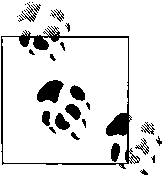
\includegraphics[width=2cm,clip]{paipai.png}
\end{wrapfigure}
\mbox{}\begin{flushleft}如果你可以使用calloc()分配内存那就坚决不要使用memset()了。不要先用malloc()分配了内存,再马上使用 memset()来进行清零。虽然结果可能是一样的,但是将这两次调用合并成直接返回已经清零了的空间calloc()会更好。好处在于你不仅少了一次函数调用,而且calloc()是直接从内存中获取已经清零了的内存,这显然比手工的将每个字节清零要高效。\end{flushleft}

\subsection{字节比较}

和strcmp()相似,memcmp()比较两块内存是否相等: 

% \setmonofont{DejaVu Sans Mono}
\begin{lstlisting}
  #include <string.h>
  int memcmp (const void *s1, const void *s2, size_t n);
\end{lstlisting}

调用memcmp()比较s1和s2的头n个字节,如果两块内存相同就返回0,如果s1小于s2就返回一个小于0的数,反之则返回大于0的数。

BSD同样提供了自己具有类似功能的接口:

% \setmonofont{DejaVu Sans Mono}
\begin{lstlisting}
  #include <strings.h>
  int bcmp (const void *s1, const void *s2, size_t n);
\end{lstlisting}

调用bcmp()会比较s1和s2的前n字节,如果两块内存就一样返回0,否则返回非0值。因为结构填充的存在(参照本章之前的“其它对齐问题”),通过memcmp()或者bcmp()来比较两个结构是否相等是不可靠的。同一个结构的两个实例也可能因为有未初始化的填充内容而被判为不相等。因此,下面的代码是不安全的: 

\begin{lstlisting}
  /* are two dinghies identical? (BROKEN) */
  int compare_dinghies (struct dinghy *a, struct dinghy *b)
  {
      return memcmp (a, b, sizeof (struct dinghy));
  }
\end{lstlisting}

程序员们如果想要比较结构体,只能一个一个比较结构体中的每一个元素。下面这个方法实现了一些优化,但它的工作量当然会比不安全的memcmp()要大: 

\begin{lstlisting}
  /* are two dinghies identical? */
  int compare_dinghies (struct dinghy *a, struct dinghy *b)
  {
      int ret;
      if (a->nr_oars < b->nr_oars)
          return -1;
      if (a->nr_oars > b->nr_oars)
          return 1;
      ret = strcmp (a->boat_name, b->boat_name);
      if (ret)
          return ret;
      /* and so on, for each member... */
  }
\end{lstlisting}

\subsection{字节移动}

memmove()复制src的前n字节到dst,返回dst: 

% \setmonofont{DejaVu Sans Mono}
\begin{lstlisting}
  #include <string.h>
  void * memmove (void *dst, const void *src, size_t n);
\end{lstlisting}

同样,BSD提供了一个被批评的接口来实现相同的功能: 

% \setmonofont{DejaVu Sans Mono}
\begin{lstlisting}
  #include <strings.h>
  void bcopy (const void *src, void *dst, size_t n);
\end{lstlisting}

需要指出的是尽管两个函数的参数相同,但是它们的位置是不一样的,在bcopy()中前两个参数的位置是反的。

bcopy()和 memmove()可以安全地处理内存区域重叠问题(就是说,dst的一部分在src 里面)。例如,它们允许内存块在一个给定的区域内向上或下移动。虽然这种情况很少见,但是程序员应该知道有这么一回事。所以C标准定义了一个不支持内存区域覆盖的memmove()变种。这个变种可能会快一点: 

% \setmonofont{DejaVu Sans Mono}
\begin{lstlisting}
  #include <string.h>
  void * memcpy (void *dst, const void *src, size_t n);
\end{lstlisting}

除了dst和src间不能重叠,这个函数基本和memmove()一样。如重叠了,函数的结果是未被定义的。另外一个安全的复制函数是memccpy(): 

% \setmonofont{DejaVu Sans Mono}
\begin{lstlisting}
  #include <string.h>
  void * memccpy (void *dst, const void *src, int c, size_t n);
\end{lstlisting}

memccpy()和memcpy()类似,但当它发现字节c在src指向的前n个字节中时会停止拷贝。它返回指向dst中c后一个字节的指针,或者当没有找到c时返回NULL。

最后我们可以使用mempcpy()来跨过拷贝的内存: 

% \setmonofont{DejaVu Sans Mono}
\begin{lstlisting}
  #define _GNU_SOURCE
  #include <string.h>
  void * mempcpy (void *dst, const void *src, size_t n);
\end{lstlisting}

函数mempcpy()和memcpy()几乎一样,区别在于memccpy()返回的是指向被复制的内存的最后一个字节的下一个字节的指针。当在内存中有连续的一系列数据需要拷贝时它是很有用的。但是它并没有太大的性能提升,因为返回的指针只是dst+n而已。这个函数是GNU中特有的。 

\subsection{字节搜索}

函数memchr()和memrchr()可以在内存块中搜索一个给定的字节: 

% \setmonofont{DejaVu Sans Mono}
\begin{lstlisting}
  #include <string.h>
  void * memchr (const void *s, int c, size_t n);
\end{lstlisting}

函数memchr()从s指向的区域开的n个字节中寻找c,c将被转换为unsigned char: 

% \setmonofont{DejaVu Sans Mono}
\begin{lstlisting}
  #define _GNU_SOURCE
  #include <string.h>
  void * memrchr (const void *s, int c, size_t n);
\end{lstlisting}

函数返回指向第一个匹配c的字节的指针,如果没找到c则返回NULL。

memrchr()与memchr()类似,不过它是从s指向的内存开始反向搜索n个字节。和memchr()不同,memrchr()是GNU的扩展函数,而不是C语言的一部分。 对于更加复杂的搜索,有个名字很烂的memmem()函数,它可以在一块内存中搜索任意的字节数组: 

% \setmonofont{DejaVu Sans Mono}
\begin{lstlisting}
  #define _GNU_SOURCE
  #include <string.h>
  void * memmem (const void *haystack,
                 size_t haystacklen,
                 const void *needle,
                 size_t needlelen);
\end{lstlisting}

memmem()函数在指向长为haystacklen的内存块haystack中查找,并返回第一块和长为needlelen的needle匹配的子块的指针。如果函数在haystack中不能找到needle,它会返回NULL。这个函数同样是GNU的扩展函数。 

\subsection{字节加密}

Linux的C库提供了进行简单数据加密的接口:

% \setmonofont{DejaVu Sans Mono}
\begin{lstlisting}
  #define _GNU_SOURCE
  #include <string.h>
  void * memfrob (void *s, size_t n);
\end{lstlisting}

memfrob()函数将s指向的位置开始的n个字节,每个都与42进行异或操作来对数据进行加密。函数返回s。

再次对相同的区域调用memfrob()可以将其转换回来。因此下面这行程序对于secret没有进行什么实质性的操作: 

\begin{lstlisting}
  memfrob (memfrob (secret, len), len);
\end{lstlisting}

这个函数用于数据加密时绝对不合适的(甚至是更差的);它的使用仅限于对于字符串的简单处理。它是GNU标准函数。 

\section{内存锁定}

Linux 实现了请求页面调度,页面调度是说在需要时将页面从硬盘交换进来,当不再需要时再交换出去。这使得系统中进程的虚拟地址空间与实际的物理内存大小没有直接的关系,同时硬盘上的交换空间提供一个拥有近乎无限物理内存的假象,

交换对进程来说是透明的,应用程序一般都不需要关心(甚至不需要知道)内核页面调度的行为。然而,在下面两种情况下,应用程序可能希望影响系统的页面调度: 

\begin{eqlist*}
\item[确定性(Determinism)] 时间约束严格的应用程序需要自己来决定页的调度行为。如果一些内存操作引起了页错误-这会导致昂贵的磁盘操作-应用程序则可能会超出要求的运行时间。如果能确保需要的页面总在内存中且从不被交换进磁盘,应用程序就能保证内存操作不会导致页错误,提供一致的,可确定的程序行为,从而提供了效能。 
\item[安全性(Security)]如果内存中含有私人信息,这些信息可能最终被页面调度以不加密的方式储存到硬盘上。例如,如果一个用户的私钥正常情况下是以加密的方式保存在磁盘上的,一个在内存中未加密的密钥备份最后可能保存在了交换文件中。在一个高度注重安全性的环境中,这样做可能是不可接受。这样的应用程序可以请求将密钥一直保留在物理内存上。
\end{eqlist*}

当然,改变内核的行为可能会对系统整体的表现产生负面的影响。应用的确定性和安全性可能会提高,但是当它的页被锁在了内存中,那另一个应用的页就只能被换出内存。如果我们相信内核的设计,那么它将总是把最优的页换出,也就是那些在未来最有可能被访问的页。因此如果你改变的它的行为,那么它就只能将一个次优的页换出了。

\subsection{锁定部分地址空间}

POSIX1003.1b-1993定义两个接口将一个或更多的页面“锁定”在物理内存,来保证它们不会被交换到磁盘。第一个函数锁定给定的一个地址区间: 

% \setmonofont{DejaVu Sans Mono}
\begin{lstlisting}
  #include <sys/mman.h>
  int mlock (const void *addr, size_t len);
\end{lstlisting}

调用mlock()将锁定addr开始长度为len个字节的虚拟内存。成功的话,函数返回0;失败时,函数返回-1,并适当设置errno。

成功调用会将所有包含[addr,addr+len)的物理内存页锁定。例如,一个调用只是指定了一个字节,包含这个字节的所有物理页都将被锁定。POSIX标准要求addr应该与页边界对齐。Linux并没有强制要求,如果真要这样做的时候,会悄悄的将addr向下调整到最近的页面。对于要求可移植到其它系统的程序需要保证addr是页对齐的。

合法的errno包括: 

\begin{eqlist*}
\item[EINVAL] 参数len是负数。 
\item[ENOMEM] 函数尝试锁定多于RLIMIT\_MEMLOCK限制的页(详见之后“锁定限制”部分)。
\item[EPERM] RLIMIT\_MEMLOCK是0,但进程并没有CAP\_IPC\_LOCK权限。(同样请见“锁定限制”部分)。
\end{eqlist*}

\begin{wrapfigure}{l}{2.5cm}
  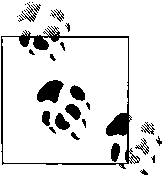
\includegraphics[width=2cm,clip]{paipai.png}
\end{wrapfigure}
\mbox{}\begin{flushleft}一个由fork()产生的子进程并不从父进程处继承锁定的内存。然而,由于Linux对地址空间写时复制机制,子进程的页面被锁定在内存中直到子进程对它们执行写操作。 \end{flushleft}

下面这个例子,假设一个程序在内存中有一个加密的字符串。一个进程可以通过下面代码来锁定拥有这个字符串的页: 

\begin{lstlisting}
  int ret;
  /* lock 'secret' in memory */
  ret = mlock (secret, strlen (secret));
  if (ret)
     perror ("mlock");
\end{lstlisting}

\subsection{锁定全部地址空间}

如果一个进程想在物理内存中锁定它的全部地址空间,使用mlock()就不再合适了。POSIX定义了mlockall()函数来满足这个实时应用中常见的需求: 

% \setmonofont{DejaVu Sans Mono}
\begin{lstlisting}
  #include <sys/mman.h>
  int mlockall (int flags);
\end{lstlisting}

mlockall()函数锁定一个进程在现有地址空间在物理内存中的所有页面。flags参数,是下面两个值的按位或操作,用以控制函数行为: 

\begin{eqlist*}
\item[MCL\_CURRENT] 如果设置了该值,mlockall()会将所有已被映射的页面(包括栈,数据段,映射文件)锁定进程地址空间中。 
\item[MCL\_FUTURE] 如果设置了该值,mlockall()会将所有未来映射的页面也锁定到进程地址空间中。
\end{eqlist*}

大部分应用程序都会同时设定这两个值。成功时,函数返回0;失败时,返回-1,并设置errno为下列错误码之一: 

\begin{eqlist*}
\item[EINVAL] 参数len是负数。
\item[ENOMEM] 函数要锁定的页面数比RLIMIT\_MEMLOCK限制的要多(详见之后“锁定限制”部分)。
\item[EPERM] RLIMIT\_MEMLOCK是0,但进程并没有CAP\_IPC\_LOCK权限。(同样请见“锁定限制”部分)。
\end{eqlist*}

\subsection{内存解锁}

POSIX标准提供了两个接口用来将页从内存中解锁,允许内核根据需要将页换出至硬盘中: 

% \setmonofont{DejaVu Sans Mono}
\begin{lstlisting}
  #include <sys/mman.h>
  int munlock (const void *addr, size_t len);
  int munlockall (void);
\end{lstlisting}

系统调用munlock()解除addr开始长为len的内存所在的页面地锁定。它消除mlock()的效果。而munlockall()则消除mlockall()的效果。两个函数在成功时都返回0,失败时返回-1,像如下设置errno: 

\begin{eqlist*}
\item[EINVAL] 参数 len 是负数(仅对munlock())。
\item[ENOMEM] 被指定的页面中有些是不合法的。
\item[EPERM] RLIMIT\_MEMLOCK是0,但进程并没有CAP\_IPC\_LOCK权限。(同样请见“锁定限制”部分)。
\end{eqlist*}

内存锁定并不会重叠。所以,不管被mlock()或mlockall()锁定了多少次,仅一个mlock()或者munlock(),即会解除一个页面的锁定。 

\subsection{锁定的限制}

因为内存的锁定能影响一个系统的整体性能-实际上,如果太多的页面被锁定,内存分配会失败------Linux对于一个进程能锁定的页面数进行了限制。

拥有CAP\_IPC\_LOCK权限的进程能锁定任意多的页面。没有这个权限的进程只能锁定RLIMIT\_MEMLOCK个字节。默认情况下,该限制是32KB(足够将一两个秘密信息锁定在内存中)对系统性能也没有什么负面影响。(第6章讨论资源限制和怎样找到和设置这些值) 

\subsection{这个页面在物理内存中吗?}

出于调试的需要,Linux提供了mincore()函数,可以用来确定一个给定范围内的内存是在物理内存中还是被交换到了硬盘中: 

% \setmonofont{DejaVu Sans Mono}
\begin{lstlisting}
  #include <unistd.h>
  #include <sys/mman.h>
  int mincore (void *start,
               size_t length,
               unsigned char *vec);
\end{lstlisting}

调用mincore()提供了一个向量,表明调用时刻映射中哪个页面是在物理内存中。函数通过vec来返回向量,这个向量描述start(必需页面对齐)开始长为length(不需要对其)字节的内存中的页面的情况。vec的每个字节对应指定区域内的一个页面,第一个字节对应着第一个页面,然后依次对应。因此,vec必须足够大来装入(length-1+page size)/page size字节。如果那页面在物理内存中,对应字节的最低位是1,否则是0。其它的位目前还没有定义,留待日后使用。

成功时,函数返回0。失败时,返回-1,并设置errno为如下值之一: 

\begin{eqlist*}
\item[EAGAIN] 内核目前没有足够的可用资源来满足请求。
\item[EFAULT] 参数vec指向一个非法地址。
\item[EINVAL] 参数start不是页对齐。
\item[ENOMEM] [address,address+1) 中的内存不在某个基于文件的映射中。
\end{eqlist*}

目前来说, 这个系统调用只能用在以MAP\_SHARED创建的基于文件的映射上。这在很大程度上限制了这个函数的使用。 

\section{投机性存储分配策略}

Linux 使用投机分配策略。当一个进程向内核请求额外的内存-如扩大它的数据段,或者创建一个新的存储器映射-内核作出了分配承诺但实际上并没有分给进程任何的物理存储。仅当进程对新“分配到”的内存区域作写操作的时候,内核才履行承诺,分配一块物理内存。内核逐页完成上述工作,并在需要时进行请求页面调度和写时复制。

这样处理有如下几个优点。首先,延缓内存分配允许内核将大部分工作推迟到最后一刻(当确实需要进行分配时)。第二,由于请求是根据需求逐页的分配,只有真正需要物理内存的时候才会消耗物理存储。最后,分配到的内存可能比实际的物理内存甚至比可用的交换空间多得多。最后这个特征叫做超量使用(overcommitment)。 

\subsection{超量使用和内存耗尽}

和在应用请求页面就分配物理存储相比,在使用时刻才分配物理存储的过量使用机制允许系统运行更多,更大的应用程序。如果没有超量使用,用写时复制映射2GB文件需要内核划出2GB的物理存储。采用超量使用,映射2GB文件需要的存储量仅仅是进程映射区域中真正进行写操作的所有页面的大小。同样,没有超量使用,就算大多数页面都不需要进行写时拷贝,每个fork()操作都需要申请空闲内存来复制整个地址空间。

但是,如果系统中的进程为满足超量使用而申请的内存大于物理内存和交换空间之和,这时会怎样呢?在这种情况下,一个或者更多的分配一定会失败。因为内核已经承诺给进程分配内存了(系统调用成功返回),而这个进程尝试使用已分配的内存,内核只能杀死另一个进程并释放它的内存,以此来满足下一次的分配需求。

当超量使用导致内存不足以满足一个请求时,我们就说发生了内存耗尽(OOM)(out of memory)。为了处理OOM,内核使用OOM 终结者(killer)来挑选一个进程,并终止它。基于这个目的,内核会尝试选出一个最不重要且又占用很多内存的进程。

OOM 其实很少出现-所以采用效果非凡的超量使用非常有实际意义的。然而,可以肯定的是,没人希望发生OOM,而且进程突然被OOM 终结者(killer)终结了也往往是无法接受。

对于不想这种情况出现的系统,内核允许通过文件/proc/sys/vm/overcommit\_memory关闭超量使用,和此功能相似的还有sysctl的vm.overcommit\_memory参数。

参数的默认值是0,告诉内核执行适度的超量使用策略,在合理范围内实施超量使用,超出限定值时则不可使用。值为1时,确认所有的分配请求,将一切顾虑抛诸脑后。一些对存储要求较高的应用程序,(例如在科学计算领域)倾向于请求比他们实际需要更多的内存,这时这个参数值就很有帮助。

当值为2时,关闭所有的过量使用,启用严格审计(strict accounting)策略。这个模式中,承诺的内存大小被严格限制在交换空间大小加上可调比例的物理内存大小。这个比例可以在文件/proc/sys/vm/overcommit\_ratio里面设置,作用和vm.overcommit\_ratio的sysctl参数相似。 默认是50,限制承诺的内存总量是交换空间加上物理内存的一半。因为物理内存还必须包含着内核,页表,系统保留页,锁定页等等东西。仅它的一部分能被交换和满足承诺请求。

使用严格审计策略时要非常小心!许多系统设计者,被OOM终结者(killer)的思想,搞得崩溃了,认为严格审计才是解决之道。然而,应用程序常常进行一些不必要的、且只有使用超量使用才能满足的分配请求,而允许这种行为也是设计虚拟内存的主要动机之一。 
